% Basic stuff
\documentclass[a4paper,10pt]{article}
\usepackage[nswissgerman]{babel}

% 3 column landscape layout with fewer margins
\usepackage[landscape, left=0.75cm, top=1cm, right=0.75cm, bottom=1.5cm, footskip=15pt]{geometry}
\usepackage{flowfram}
\ffvadjustfalse
\setlength{\columnsep}{1cm}
\Ncolumn{3}

% define nice looking boxes
\usepackage[many]{tcolorbox}

% a base set, that is then customised
\tcbset {
  base/.style={
    boxrule=0mm,
    leftrule=1mm,
    left=1.75mm,
    arc=0mm, 
    fonttitle=\bfseries, 
    colbacktitle=black!10!white, 
    coltitle=black, 
    toptitle=0.75mm, 
    bottomtitle=0.25mm,
    title={#1}
  }
}

\definecolor{brandblue}{rgb}{0.34, 0.7, 1}
\newtcolorbox{mainbox}[1]{
  colframe=brandblue, 
  base={#1}
}

\newtcolorbox{subbox}[1]{
  colframe=black!20!white,
  base={#1}
}

% Mathematical typesetting & symbols
\usepackage{amsthm, mathtools, amssymb} 
\usepackage{marvosym, wasysym}
\usepackage{derivative}
\allowdisplaybreaks

% Tables
\usepackage{tabularx, multirow}
\usepackage{booktabs}

% Make enumerations more compact
\usepackage{enumitem}
\setitemize{itemsep=0.5pt}
\setenumerate{itemsep=0.75pt}

% To include sketches & PDFs
\usepackage{graphicx}

% For hyperlinks
\usepackage{hyperref}
\hypersetup{
  colorlinks=true
}

% Metadata
\title{Cheatsheet Analysis 2}
\author{Thomas Gassmann}
\date{January 2023}

% Math helper stuff
\def\limn{\lim_{n\to \infty}}
\def\limxo{\lim_{x\to 0}}
\def\limxi{\lim_{x\to\infty}}
\def\limxn{\lim_{x\to-\infty}}
\def\sumk{\sum_{k=1}^\infty}
\def\sumn{\sum_{n=0}^\infty}
\def\R{\mathbb{R}}
\def\C{\mathbb{C}}
\def\Q{\mathbb{Q}}
\def\N{\mathbb{N}}
\def\X{\mathcal{X}}
\def\dx{\text{ d}x}

\begin{document}

\begin{center}
    Lizenziert unter CC BY-SA 4.0. Für Urheber, Quellen und Lizenzinformationen, siehe:\\
    \href{https://github.com/thomasgassmann/eth-summaries}{thomasgassmann/eth-summaries}
  \end{center}

\section{Differentialgleichungen}
\begin{mainbox}{Definition lineare DGL}
  Eine gewöhnliche lineare Differentialgleichung ist eine Gleichung, welche Ableitungen enthält. Sie hat die Form \[y^{(n)} + a_{n-1} y^{(n-1)} + \cdots + a_0y = b(x)\]
  wo die Koeffizienten \(a_0, \ldots, a_{n-1}\) komplexe Funktionen auf \(I \subset \R\) sind, welche von \(y\) abhängig sein können. Wenn \(b(x) = 0\) gilt, ist die DGL homogen.
\end{mainbox}

\begin{subbox}{Hauptresultat über Lineare ODEs}
  Sei $I \subseteq \mathbb{R}$ ein offenes Intervall und $y^{(k)} + a_{k-1} y^{(k-1)} + \cdots + a_0 y = b$ eine lineare ODE über $I$ mit stetigen Koeffizienten.
  \begin{itemize}
    \item Sei $S_0$ die Menge der Lösungen für $b = 0$ (assoziierte homogene ODE). Dann ist $S_0$ ein Vektorraum der Dimension $k$. Wenn $f_1, \cdots, f_k$ Lösungen sind, dann auch $\alpha_1 f_1 + \cdots \alpha_k f_k$ Lösungen.
    \item Für jedes $x_0 \in I$ und jedes $(y_0, \cdots, y_{k-1}) \in \mathbb{C}^k$ gibt es ein eindeutiges $f \in S_0$ mit $f(x_0) = y_0, f'(x_0) = y_1, \cdots$.
    \item Für jedes $b(x)$ ist die Menge der Lösungen $S_b = \{f + f_p | f \in S_0\}$ wobei $f_p$ eine partikuläre Lösung ist.
    \item Für jedes $x_0 \in I$ und jedes $(y_0, \cdots, y_{k-1}) \in \mathbb{C}^k$ gibt es ein eindeutiges $f \in S_b$ mit $f(x_0) = y_0, f'(x_0) = y_1, \cdots$.
  \end{itemize}
\end{subbox}

Die Menge $S$ an Lösungen ist ein Subset des Raums der komplexen Funktionen auf $I$ mit Dimension $n$.\\
\(S_0\) ist das Set der Lösungen zu einer homogenen DGL.

\subsubsection*{Lineare DGL erkennen}
\begin{itemize}
  \item keine Koeffizienten vor der höchsten Ableitung
  \item alle Koeffizienten sind stetige Funktionen
  \item keine Produkte von $y$ oder deren Ableitungen
  \item keine Potenzen von $y$ oder deren Ableitungen
  \item keine Funktionen von $y$ oder deren Ableitungen
\end{itemize}

\subsection{Lineare DGL erster Ordnung}
Wir betrachten DGL der Form \[y' + a(x)y = b(x)\]
\begin{enumerate}
  \item (Homogene Lösung) 
  \begin{align*}
    y' + a(x)y &= 0\\
    \frac{y'}{y} &= -a(x)\\
    \ln(y) &= -A(x)+C\\
    y &= e^{-A(x)+C} = z \cdot e^{-A(x)}\quad z \in \C
  \end{align*}
  \item (partikuläre Lösung) Verwende entweder ``Variation der Konstanten'' oder ``Fundiertes Raten''.
\end{enumerate}
\subsection{Variation der Konstanten}
Wir nehmen an, dass die partikuläre Lösung die homogene Lösung imitiert. Sei \(f_p = z(x)e^{-A(x)}\) für eine Funktion \(z: I \to \C\). Dann ist \(z'(x) = b(x) e^{A(x)}\) (einsetzen in DGL!) und somit \[z(x) = \int_{x_0}^x b(t) e^{A(t)} \mathop{dt}\] Daraus erhalten wir \[f_p = \int_{x_0}^x b(t) e^{A(t)} \mathop{dt} \cdot e^{-A(t)}\]

\subsection{Fundiertes Raten}

Wir nehmen an, dass die partikuläre Lösung $b$ imitiert. Wenn $b(x)$ von einer bestimmten Form ist, versuchen wir folgende $f_p$, wobei wir unseren Versuch in die DGL einsetzen, was uns dann ein Gleichungssystem für die Konstanten gibt:

\begin{center}
  \renewcommand*{\arraystretch}{1.1}
  \begin{tabular}{cc}
    \toprule
    $b(x)$ & Raten \\ 
    \midrule
    $a \cdot e^{\alpha x}$ & $b \cdot e^{\alpha x}$\\
    \hline
    $a \sin(\beta x)$ & $c \sin(\beta x) + d \cos(\beta x)$\\
    \hline
    $b \cos(\beta x)$ & $c \sin(\beta x) + d \cos(\beta x)$\\
    \hline
    $a e^{\alpha x} \sin(\beta x)$ & $e^{\alpha x} \Big( c \sin(\beta x) + d \cos(\beta x) \Big)$\\
    \hline
    $b e^{\alpha x} \cos(\beta x)$ & $e^{\alpha x} \Big( c \sin(\beta x) + d \cos(\beta x) \Big)$\\
    \hline
    \begin{tabular}{@{}c@{}}$P_n(x) e^{\alpha x}$ \\ $P_n(\alpha) \neq 0$\end{tabular} & $R_n(x) e^{\alpha x}$\\
    \hline
    \begin{tabular}{@{}c@{}}$P_n(x) e^{\alpha x}$ \\ $(x - \alpha)^m | P_n(x)$\end{tabular} & $R_n(x) x^m e^{\alpha x}$\\
    \hline
    \begin{tabular}{@{}c@{}}$P_n(x) \sin(\alpha x)$ \\ $P_n(i \alpha) \neq 0$\end{tabular} & $R_n(x) \sin(\alpha x) + S_n(x) \cos(\alpha x)$\\
    \hline
    \begin{tabular}{@{}c@{}}$P_n(x) \cos(\alpha x)$ \\ $P_n(i \alpha) \neq 0$\end{tabular} & $R_n(x) \sin(\alpha x) + S_n(x) \cos(\alpha x)$\\
    \hline
    \begin{tabular}{@{}c@{}}$P_n(x) \sin(\alpha x)$ \\ $(x - i \alpha)^m | P_n(x)$\end{tabular} & $R_n(x) x^m \sin(\alpha x) + S_n(x) x^m \cos(\alpha x)$\\
    \hline
    \begin{tabular}{@{}c@{}}$P_n(x) \cos(\alpha x)$ \\ $(x - i \alpha)^m | P_n(x)$\end{tabular} & $R_n(x) x^m \sin(\alpha x) + S_n(x) x^m \cos(\alpha x)$\\
    \hline
    $P_n e^{\alpha x} \sin(\beta x)$ & $e^{\alpha x} \left( R_n \sin(\beta x) + S_n \cos(\beta x) \right)$\\
    \hline
    $P_n e^{\alpha x} \cos(\beta x)$ & $e^{\alpha x} \left( R_n \sin(\beta x) + S_n \cos(\beta x) \right)$\\
    \bottomrule
  \end{tabular}
\end{center}

\(P_n, R_n \) und \(S_n\) sind Funktionen von \(x\). 

\begin{enumerate}
  \item Wenn \(b(x)\) eine Linearkombination der Basisfunktionen ist, dann versuche eine Linearkombination. Partikuläre Lösungen können auch separat gefunden werden und danach addiert werden.
  \item Wenn die geratene Lösung der homogenen Lösung entspricht, dann multipliziere mit \(x^m\), wobei \(m\) die Vielfachheit der Wurzel ist.
\end{enumerate}

\subsection{Lineare DGL mit konstanten Koeffizienten}
Wir betrachten DGL der Form
\[y^{(k)} + a_{k-1} y^{(k-1)} + \ldots + a_1 y' + a_0 y = b(x)\]
Wir suchen eine homogene Lösung der Form \(e^{\lambda x}\). Jetzt können wir das charakteristische Polynom lösen:
\begin{align*}
  P(\lambda) = e^{\lambda x} \left(\lambda^k + a_{k-1}\lambda^{k-1} + \ldots + a_0\right) = 0 \\ 
  \implies 0 = \lambda^k + a_{k-1}\lambda^{k-1} + \ldots+ a_0
\end{align*}

Die Nullstellen von \(P(\lambda)\) sind Eigenwerte \(\lambda_i\), mit dazugehöriger Multiplizität \(m_r\). Nun spannen die Funktionen \(f_{i,r} : x \to x^r e^{\lambda_i x}\) den Raum der Lösungen \(S_0\) auf.

Falls \(\lambda = \beta + \gamma i\) eine komplexe Nullstelle von \(P(\lambda)\) ist, so ist auch 
\(\bar{\lambda} = \beta - \gamma i\) eine Nullstelle. Daher sind \(f_1 = e^{\lambda x}\) und \(f_2 = e^{\bar{\lambda} x}\) Lösungen und können durch eine Linearkombination von \(\tilde{f_1} = e^{\beta x} \cos(\gamma x)\) und \(\tilde{f_2} = e^{\beta x} \sin(\gamma x)\) ersetzt werden.

Falls \(y^{(k)} + a_{k-1}y^{(k-1)} + \dots + a_0 y = 0\) reelle Koeffizienten hat, so führt jedes Paar von komplex konjugierten Nullstellen $\beta_j \pm \gamma_j i$ mit Multiplizität $m_j$ zu einer Lösung
\[x^l e^{\beta_j x} \Big( \cos(\gamma_j x) + i \sin(\gamma_j x) \Big) \quad \text{für }0 \leq l \leq m_j\]

Um eine partikuläre Lösung zu finden, können wir wieder fundiertes Raten oder Variation der Konstanten verwenden. 
Variation der Konstanten funktioniert wie folgt (hier 2D):

\begin{enumerate}[label=(\arabic*)]
  \item Nimm an, dass die homogene Lösung \(f = z_1 f_1 + z_2 f_2\) ist
  \item Versuche nun \(f_p = z_1(x) f_1 + z_2(x) f_2\)
  \item Löse das folgende System
  \begin{align*}
    z_1'(x) f_1 + z_2'(x) f_2 &= 0\\
    z_1'(x) f_1' + z_2'(x) f_2' &= b(x)\\
  \end{align*}
  Hier gehen wir wie folgt vor:
  \begin{align*}
    W &= f_1 f_2' - f_2 f_1' \neq 0\\
    \Rightarrow z_1' &= \frac{-f_2 b}{W} \; , z_2' = \frac{-f_1 b}{W}\\
    \Rightarrow f_p &= -f_1 \int \frac{f_2 b}{W} dt + f_2 \int \frac{f_1 b}{W} dt
  \end{align*}
\end{enumerate}

\section{Ableitungen in \texorpdfstring{\(\R^n\)}{Rⁿ}}
\begin{subbox}{Monom}
  Ein Monom vom Grad \(e\) ist
  \begin{align*}
    (x_1, \ldots, x_n) \mapsto x_1^{d_1}\cdot \ldots \cdot x_n^{d_n} \\
    e = d_1 + \ldots + d_n 
  \end{align*}
  \(\to\) ein Polynom, das nur aus einem Glied besteht.
\end{subbox}
\begin{mainbox}{Polynom}
  Ein Polynom mit \(n\) Variablen vom Grad \(d\) ist eine endliche Summe von Monomen mit Grad \(e \le d\).
\end{mainbox}

\subsection{Konvergenz}
\begin{enumerate}
  \item Skalarprodukt: \(\left< x,y\right> = \sum_{i=0} x_i \cdot y_i\)
  \item Euklidische Norm: \(||x|| := \sqrt{x_2^1 + \cdots + x_n^2}\) mit den folgenden Eigenschaften:
  \begin{enumerate}
    \item \(||x|| \ge 0, ||x|| = 0 \iff x = 0\)
    \item \(||\lambda x|| = |\lambda| \cdot ||x||, \forall \lambda \in \R\)
    \item \(||x+y|| \le ||x|| + ||y||\)
    \item \(|\left<x,y\right>| \le ||x|| \cdot ||y||\)
  \end{enumerate}
\end{enumerate}

\begin{mainbox}{Definition Konvergenz}
  Sei \((x_k)_{k \in \mathbb{N}}, x_k \in \R^n\). Die folgenden Definitionen sind für \(\lim_{k\to\infty}x_k = y\) äquivalent:
  \begin{enumerate}
    \item \(\forall \epsilon > 0 \exists N \ge 1\) so dass \(\forall k \ge N \ ||x_k - y|| < \epsilon\).
    \item Für jedes \(i, 1 \le i \le n\) konvergiert die Folge \((x_{k,i})_k\) von reellen Zahlen nach \(y_i\).
    \item Die Folge der reellen Zahlen \(||x_k - y||\) konvergiert nach \(0\).
  \end{enumerate}
\end{mainbox}
\subsection{Stetigkeit}
Sei \(f: \X \subset \R^n \to \R^m\)  und \(x_0 \in \X\). \(f\) ist stetig in \(x_0\), falls eine der folgenden Bedingungen erfüllt ist:
\begin{enumerate}
  \item \(\forall \epsilon > 0 \exists \delta > 0\) so dass \(x \in \X ||x - x_0|| < \delta \implies ||f(x) - f(x_0)|| < \epsilon\).
  \item \(\forall\) Folgen \((x_k)\) in \(X\) mit \(\lim x_k = x_0\) gilt \(\lim f(x_k) = f(\lim x_k)\).
\end{enumerate}
\(f\) ist stetig in \(\X\) falls \(f\) für jeden Punkt \(x_0 \in \X\) stetig ist. Es gilt:
\begin{enumerate}
  \item \(f(x = x_1, \ldots, x_n) \mapsto (f_1(x),\ldots,f_m(x))\) und \(f_i: \R^n \to \R\) stetig \(\iff \forall i = 1, \ldots, m \ f_i\) stetig.
  \item Lineare Funktionen \(x \mapsto Ax\) sind stetig.
  \item Polynome sind stetig.
  \item Summen + Produkte von stetigen Funktionen sind stetig.
  \item Funktionen unterschiedlicher Variablen sind stetig, falls alle Variablen stetig sind.
  \item Verknüpfungen stetiger Funktionen sind stetig.
\end{enumerate}
\begin{mainbox}{Sandwich-Lemma}
  Wenn \(f, g, h: \R^n \to \R\) Funktionen mit \(f(x) < g(x) < h(x) \forall x \in \R^n\) sind, dann gilt
  \[\lim_{x\to a} f(x) = \lim_{x \to a} h(x) = L \implies \lim_{x\to a} g(x) = L\]
\end{mainbox}
\subsection{Eigenschaften von Mengen}
Eine Menge \(\X \subset \R^n \) ist
\begin{itemize}
  \item \textbf{beschränkt}, falls die Menge \(\{ ||x|| \mid x \in \X \}\) in \(\R\) beschränkt ist (d.h. \(\exists R \ge 0, \forall x \in \X: ||x|| \le R\)).
  \item \textbf{abgeschlossen}, falls jede Folge \((x_k)_{k\in \N} \subset \X\), die in \(\R^n\) konvergiert, zu einem Punkt in \(y \in \X\) konvergiert. Dies kann mit einem Ball visualisiert werden. Gegenbeispiele: \(\frac{1}{k}, <\).
  \item \textbf{kompakt}, falls sie beschränkt und abgeschlossen ist.
  \item \textbf{offen}, falls ihr Komplement \(\R^n \setminus \X\) abgeschlossen ist.
  \item \textbf{konvex}, falls \(\forall x, y \in \X: \lambda x + (1 - \lambda)y \in \X\) gilt (die Linie zwischen \(x, y\) ist in \(\X\)).
\end{itemize}
Beispiele:
\begin{itemize}
  \item \((a,b) \subset \R\) ist offen.
  \item \(\left[a,b\right) \subset \R\) ist weder offen noch abgeschlossen.
  \item \(\R^n\) und \(\varnothing\) sind offen.
  \item \((a_1, b_1) \times (a_2,b_2) \subset \R^2\) ist offen.
  \item Urbilder von offenen Mengen sind unter stetigen Abbildungen offen. Urbilder von geschlossenen Mengen sind unter stetigen Abbildungen geschlossen. Die Umkehrung ist im Allgemeinen falsch.
\end{itemize}
\begin{subbox}{Bolzano-Weierstrass}
  Jede beschränkte Folge in \(\R^n\) hat eine konvergente Teilfolge.
\end{subbox}
\begin{subbox}{Min-Max-Theorem}
  Sei \(\X \subset \R^n, \X \ne \varnothing\) eine kompakte Menge und \(f: \X \to \R\) eine stetige Funktion. Dann ist \(f\) beschränkt und ein Maximum \(x^+\)/Minimum \(x^-\)existieren, so dass
  \[f(x^+) = \sup_{x\in \X} f(x) \quad f(x^-) = \inf_{x \in \X} f(x)\]
\end{subbox}
\subsection{Partielle Ableitungen}
Um eine partielle Ableitung von \(f: \X \subset \R^n \to \R\) (wobei \(\X\) offen) zu finden, betrachten wir alle Variablen bis auf eine als konstant und leiten nach dieser ab.
\[\pdv{f}{x_{0,j}} = \lim_{h \to 0} \frac{f(x_{0,1}, \ldots, x_{0,j} + h, \ldots, x_{0,n}) - f(x_0)}{h}\]
Für \(f: \R^n \to \R^m, x_0 \in \R^n\) gilt
\begin{align*}
  \pdv{f(x_0)}{x_j} := \begin{pmatrix}
    \pdv*{f_1(x_0)}{x_j}\\
    \vdots\\
    \pdv*{f_m(x_0)}{x_j}\\
  \end{pmatrix}
\end{align*}
Partielle Ableitungen haben folgende Eigenschaften:
\begin{enumerate}
  \item \(\partial_j(f + g) = \partial_j (f) + \partial_j g\)
  \item \(\partial_j(f \cdot g) = \partial_j (f) \cdot g + \partial_j (g) \cdot f\)
  \item \(\partial_j(f / g) = \frac{\partial_j (f) \cdot g - \partial_j (g) \cdot f}{g^2}\) für \(g \ne 0\)
\end{enumerate}
\begin{mainbox}{Jacobi-Matrix}
Sei \(f: \X \subset \R^n \to \R^m\) und \(\X\) eine offene Menge. Die Jacobi-Matrix ist eine Matrix mit \(m\) Zeilen und \(n\) Spalten:
\[J_f = \left( \pdv{f_i}{x_j} \right)_{\substack{1 \leq j \leq n \\ 1 \leq i \leq m}}\]
\end{mainbox}
\begin{mainbox}{Gradient}
  Die Jacobi-Matrix einer Funktion \(f: \X \subset \R^n \to \R\) ist ein Spaltenvektor, der mit \(\nabla f\) bezeichnet wird. Die geometrische Interpretation ist ein Vektorfeld, definiert durch \(\nabla f\), welches die Richtung und Magnitude des grössten Wachstums von \(f\) angibt.
\end{mainbox}
\begin{subbox}{Divergenz}
  Die Divergenz einer Funktion \(f\) ist die Spur der Jacobi-Matrix von \(f\). \[\text{div}(f)(x_0) = \text{Tr}(J_f(x_0)) = \sum_{i=0}(J_f)_{i,i}\]
\end{subbox}
\subsection{Differenzierbarkeit}
Sei \(f: \X \subset \R^n \to \R^m, x_0 \in \X\). \(f\) ist differenzierbar an der Stelle \(x_0\), falls eine lineare Abbildung \(L: \R^n \to \R^m\) (d.h. eine \(m \times n\)-Matrix \(L\)) existiert, so dass \(\forall x_0 + v \in \X\):
\[f(x_0 + v) = f(x_0) + L(v) + R(x_0,v)\]
wobei für den Fehlerterm \(R\) folgendes gilt: 
\[\lim_{v \to 0} \frac{||R(x_0,v)||}{||v||} = 0\]
Wir schreiben \(df(x_0) = L\). Wenn \(f\) für alle \(x_0 \in \X\) differenzierbar ist, dann ist \(f\) auf \(\X\) differenzierbar. \\
Wenn alle partiellen Ableitungen existieren und stetig sind, dann ist \(f\) differenzierbar.\\
Falls \(f,g\) im Punkt \(x_0 \in \X\) differenzierbar sind, gilt:
\begin{enumerate}
  \item \(f\) ist stetig im Punkt \(x_0\)
  \item \(f\) hat alle partiellen Ableitungen am Punkt \(x_0\) und die Matrix, welche \(df(x_0): x \mapsto Ax\) repräsentiert, ist die Jacobi-Matrix von \(f\) am Punkt \(x_0\), d.h. \(A = J_f(x_0)\)
  \item \(d(f+g)(x_0) = df(x_0) + dg(x_0)\)
  \item Wenn \(m = 1\) ist, dann ist \(f\cdot g\) differenzierbar. Wenn ausserdem \(g \ne 0\) gilt, dann ist es \(f/g\) auch.
  \item Wenn \(f: \X \to Y, g: Y \to \R^m\) beide differenzierbar sind, so gilt \(d(g \circ f)(x_0) = dg(f(x_0)) \circ df(x_0)\). 
  Weiter ist \(J_{g \circ f}(x_0) = J_g(f(x_0)) \cdot J_f(x_0)\).
  \item Äquivalent dazu: $f$ differenzierbar in $x_0$\\
  falls $\lim_{x \rightarrow x_0} \frac{f(x) - (f(x_0) + u(x - x_0))}{||x - x_0||} = 0$ für eine lineare Abbildung $u: \mathbb{R}^n \rightarrow \mathbb{R}^m$.
  \item Die Richtungsableitung $D_u f(a)$ existiert, wenn $t \mapsto f(a + tu)$ in $t = 0$ differenzierbar ist.
\end{enumerate}
Die Ableitung einer Funktion ist gegeben durch
\begin{align*}
  f'(x_0) &= \begin{pmatrix}
    f_1'(x_0)\\
    \vdots\\
    f_n'(x_0)
  \end{pmatrix}
\end{align*}
\begin{subbox}{Tagentialraum}
  Der Tangentialraum eines Graphen \(f\) am Punkt \(x_0\) ist gegeben durch \(g(x) = f(x_0) + df(x_0)(x-x_0)\).
\end{subbox}

\subsection{Level sets}

\begin{mainbox}{Level sets}
  $L_c = \{ x \in \mathbb{R}^n | f(x) = c \}$ nennt man ein Level set.
\end{mainbox}

Der Gradient an einem Punkt $x_0$ ist immer orthogonal zum Level set von $x_0$. 

\subsection{Höhere Ableitungen}
Sei \(\X \subset \R^n\) offen, \(f: \X \mapsto \R^m\). \(f\) ist eine Funktion der Klasse \(C^1\) falls \(f\) auf \(\X\) differenzierbar ist und alle partiellen Ableitungen stetig sind. \\
Allgemein gilt \(f \in \C^k\) für \(k \ge 2\) wenn \(f\) differenzierbar ist und für alle partiellen Ableitungen \(\partial_{x_i} f \in C^{k-1}\) gilt. \\
\(f\) ist glatt oder in \(C^\infty\) falls \(\forall k: f \in C^k \). Alle Polynome sind glatt.

Partielle Ableitungen bis zur Ordnung \(k\) sind kommutativ:
$$\pdv{f}{x_i, x_j} = \pdv{f}{ x_j, x_i}$$

\begin{mainbox}{Hesse-Matrix}
  Die Hesse-Matrix ist eine \(n \times n\) symmetrische Matrix, welche die zweite Ableitung definiert:
  \[\text{Hess}_f(x_0) := \left(\pdv{f(x_0)}{x_i, x_j}\right)_{1\le i,j \le n}\] 
\end{mainbox}
\subsection{Taylorpolynome}
Sei \(k \le 1\) und \(f: \X \mapsto \R\) ist eine Funktion der Klasse \(C^k\) auf \(\X\). Sei \(x_0 \in \X\) fix. Das \(k\)-te Taylorpolynom von \(f\) am Punkt \(x_0\) ist das Polynom in \(n\) Variablen vom Grad \(\le k\):
\begin{align*}
  &T_k f(y; x_0) = f(x_0) + \sum_{i=1}^n \partial_i f(x_0) \cdot y_i + \dots \\
  &+ \sum_{m_1 + \cdots + m_n = k} \frac{1}{m_1! \cdots m_n!} \pdv{^k f(x_0) }{x_1^{m_1} \cdots \partial x_n^{m_n}} \cdot y_1^{m_1} \cdots y_n^{m_n}
\end{align*}

\subsubsection*{Beispiele}
\begin{align*}
  T_1 f(\vec{x}; x_0) &:= f(x_0) + \nabla f(x_0) \cdot \vec{x} \\
  T_2 f(\vec{x}; x_0) &:= T_1f + \frac{1}{2} \cdot \vec{x}^\top \cdot \text{Hess}_f(x_0) \cdot \vec{x}
\end{align*}

\subsection{Definit}
Eine symmetrische Matrix ist
\begin{itemize}
  \item \textbf{positiv definit}, falls alle Eigenwerte positiv sind.
  \item \textbf{negativ definit}, falls alle Eigenwerte negativ sind.
  \item \textbf{indefinit}, falls sowohl positive als negative Eigenwerte existieren.
\end{itemize}
Eigenwerte können mit dem charakteristischen Polynom gefunden werden:
\begin{align*}
  \text{det} \left(
  \begin{pmatrix}
    a & b\\
    c & d
  \end{pmatrix}
  -
  \begin{pmatrix}
    \lambda & 0\\
    0 & \lambda
  \end{pmatrix}
  \right)
  &=
  \text{det}
  \begin{pmatrix}
    a - \lambda & b\\
    c & d - \lambda
  \end{pmatrix}\\
  &\Rightarrow ad - (a + d) \lambda + \lambda^2 - bc = 0
\end{align*}
Für nichtsymmetrische Matrizen müssen wir für jeden Vektor \(v\) testen, ob \(v^\top A v > 0\) (bzw. \(< 0\)) gilt.
\subsubsection*{Determinante in drei Dimensionen}
\begin{align*}
  a \cdot \text{det}
  \begin{pmatrix}
    e & f\\
    h & i
  \end{pmatrix}
  - b \cdot \text{det}
  \begin{pmatrix}
    d & f\\
    g & i
  \end{pmatrix}
  + c \cdot \text{det}
  \begin{pmatrix}
    d & e\\
    g & h
  \end{pmatrix}
\end{align*}
\subsection{Extrema}
\subsubsection*{Lokale Extrema}
Sei \(f: \X \subset \R^n \mapsto \R\) differenzierbar und \(\X\) eine offene Menge. Dann ist \(x_0 \in \X\) ein lokales Maximum (Minimum) falls wir eine Umgebung \(B_r(x_0) = \{x\in \R^n \mid ||x-x_0|| < r \} \subset \X\) finden können, wo gilt:
\[\forall x \in B_r(x_0): f(x) \le (\ge) f(x_0)\]
Wenn \(x_0 \in \X\) ein lokales Extrema ist, dann gilt ausserdem \(\nabla f(x_0) = 0\).

\subsubsection*{Kritische Punkte}
Ein Punkt \(x_0 \in \X\) wo \(\nabla f(x_0) = 0\) gilt ist ein kritischer Punkt. Wenn \(\det(\text{Hess}_f(x_0)) \ne 0\), dann ist \(x_0\) nicht-degeneriert.

\subsubsection*{Sattelpunkt}
Wenn ein kritischer Punkt weder Maximum noch Minimum ist, dann nennen wir ihn Sattelpunkt.

\subsubsection*{Globale Extrema}
Sei \(f: K \mapsto \R\) und \(K\) kompakt, dann existiert ein globales Extrema von \(f\) und es ist entweder ein kritischer Punkt oder am Rand von \(K\). Um ein solches Extrema zu bestimmen, teilen wir \(K\) in sein Inneres \(\X\) und den Rand \(B\) auf. 

Nun bestimmen wir zuerst wie zuvor die kritischen Punkte von \(\X\). Um die Maximas/Minimas von \(B\) zu bestimmen, benötigen wir nur Wissen aus Analysis I (da von der Form \(\R \mapsto \R\)).
\subsubsection*{Testen von kritischen Punkten}
Sei \(f: \X \subseteq \R^n \mapsto \R, \X\) offen und \(f\in C^2\). Sei \(x_0\) ein nicht-degenerierter kritischer Punkt von \(f\). Dann gilt:
\begin{enumerate}
  \item $\text{Hess}_f(x_0)$ pos. def. \(\implies\) $x_0$ ist lokales Minimum.
  \item $\text{Hess}_f(x_0)$ neg. def. \(\implies\) $x_0$ ist lokales Maximum.
  \item $\text{Hess}_f(x_0)$ indefinit \(\implies\) $x_0$ ist Sattelpunkt.
\end{enumerate}
Dies funktioniert nicht, wenn \(x_0\) ein degenerierter kritischer Punkt ist. In einem solchen Fall müssen die Vorzeichen überprüft werden.
\subsubsection*{Kritische Punkte mit Nebenbedingungen}
Wenn wir Minimas/Maximas einer Funktion \(f: \X \mapsto \R\) mit einer Nebenbedingung \(g(x) = 0, g: \X \mapsto \R\) bestimmen wollen, können wir dafür Lagrange-Multiplikatoren verwenden.
\begin{subbox}{Lagrange-Multiplikator}
  Sei \(\X \subset \R^n\) offen und \(f,g: \X \mapsto \R\) Funktionen der Klasse \(C^1\). Wenn \(Y = \{x \in \X \mid g(x) = 0\) ist, dann ist \(x_0 \in Y\) ein lokales Extrema, welches die Nebenbedingung erfüllt, falls 
  \[\exists \delta > 0, f(y) \le (\ge) f(x_0), \quad \forall y \in B_\delta(x_0) \cap Y\]
  gilt. Nun ist entweder \(\nabla g(x_0) = 0\) oder \(\exists \lambda \in \R, \nabla f(x_0) = \lambda \cdot \nabla g(x_0)\), wobei \(\lambda\) dann Lagrange-Multiplikator gennant wird.
\end{subbox}
\section{Integrale in \texorpdfstring{\(\R^n\)}{Rⁿ}}
\subsection{Einfache Integrale}
Für \(f: \R \mapsto \R^n\) ist das Integral definiert als
\[\int_a^b f(t)dt = 
\begin{pmatrix*}
  \int_a^b f_1(t) dt \\
  \vdots\\
  \int_a^b f_n(t) dt
\end{pmatrix*}
\]

\begin{mainbox}{Kurve}
  Eine parametrisierte Kurve in \(\R^n\) ist eine stetige Ableitung \(\gamma: \left[a,b\right] \mapsto \R^n\) wobei \(\gamma\) stückweise in \(C^1\) ist, d.h. wir können \(\gamma\) so partitionieren, das alle Partitionen in \(C^1\) sind. Eine parametrisierte Kurve muss nicht injektiv sein.
\end{mainbox}
\subsection{Wegintegrale}
Sei \(\gamma : \left[a,b\right] \mapsto \R^n\) eine parametrisierte Kurve und \(\X \subset \R^n\) eine Menge, welche das Bild von \(\gamma\) beinhaltet. Sei \(f : \X \mapsto \R^n\) eine stetige Funktion. Dann ist ein Wegintegral (auch: Kurvenintegral) definiert als:
\[\int_\gamma f(s) ds = \int_a^b f(\gamma(t)) \cdot \gamma'(t) dt\]

Wegintegrale haben folgende Eigenschaften:
\begin{enumerate}
  \item Sie sind unabhängig von orientierungserhaltenden Reparametrisierungen, d.h. sie hängen nur vom Bild der Kurve und nicht von der Parametrisierung ab.
  \begin{align*}
    \gamma&: [a,\, b] \mapsto \R^n\\
    \tilde{\gamma}&: [c,\, d] \mapsto \R^n\\
    \varPhi&: [c, \, d] \mapsto [a, \, b]\\
    \tilde{\gamma} &= \gamma \circ \varPhi = \gamma(\varPhi)\\
    \Rightarrow &\int_\gamma f(s) \; ds = \int_{\tilde{\gamma}} f(s) \; ds
  \end{align*}
  \item Sei \(\gamma_1 + \gamma_2\) ein Pfad gegeben durch die Vereinigung zweier Kurven. Dann gilt
  \begin{align*}
    \gamma_1 + \gamma_2 &:=
    \begin{cases}
      \gamma_1(t) \quad& t \in [a, \, b]\\
      \gamma_2(t) \quad& t \in [b, \, d + b - c]
    \end{cases}\\
    \int_{\gamma_1 + \gamma_2} f(s) \; ds &= \int_{\gamma_1} f(s) \; ds + \int_{\gamma_2} f(s)\; ds
  \end{align*}
  \item Sei \(\gamma : \left[a,b\right] \mapsto \R^n\) ein Pfad und \(-\gamma\) ist der Pfad in die Gegenrichtung (d.h. \((-\gamma)(t) = \gamma(a + b - t)\)). Dann gilt
  \[\int_{-\gamma} f(s)ds = -\int_\gamma f(s) ds\]
\end{enumerate}

\subsection{Potential}
Ein differenzierbares skalares Feld \(g: \X \subset \R^n \mapsto \R\) mit \(\nabla g = f, f: \X \mapsto \R^n\) wird ein \textbf{Potential} von \(f\) genannt. Dies kann wie folgt verwendet werden:
\begin{align*}
  \int_\gamma f \; ds &= \int_a^b f(\gamma(t)) \cdot \gamma'(t) \; dt\\
  &= \int_a^b \nabla g(\gamma(t)) \cdot \gamma'(t) \; dt\\
  &= \int_a^b \frac{d}{dt} (g \circ \gamma) \; dt\\
  &= (g \circ \gamma)(b) - (g \circ \gamma)(a)
\end{align*}

\subsection{Konservative Vektorfelder}
Sei \(\X\) offen und \(f: \X \subset \R^n \mapsto \R^n\) ein stetiges Vektorfeld. Die folgenden Aussagen sind äquivalent:
\begin{enumerate}
  \item Falls für irgendwelche \(x_1, x_2 \in \X\) das Wegintegral \(\int_\gamma f(s) ds\) unabhängig von der Kurve in \(\X\) von \(x_1\) nach \(x_2\) ist, dann ist das Vektorfeld \(f\) konservativ.
  \item Jedes Wegintegral in \(f\) entlang einer geschlossenen Kurve (Schlaufe) ist 0.
  \item Ein Potential für \(f\) existiert.
\end{enumerate}
Es gilt ausserdem folgende notwendige, aber nicht ausreichende Bedingung:
\[f \text{ ist konservativ }\implies \pdv{f_i}{x_j} = \pdv{f_j}{x_i}\]

\begin{subbox}{Wegzusammenhängend}
  Sei \(\X \subset \R^n\) offen. \(\X\) ist wegzusammenhängend, falls für jedes Paar an Punkten \(x, y \in \X\) ein Pfad \(\gamma : \left(0,1\right] \mapsto \X\) existiert, der in \(C^1\) ist und \(\gamma(0) = x, \gamma(1) = y\) hält.
\end{subbox}

\begin{subbox}{Sternförmig}
  Eine Teilmenge \(\X \subset \R^n\) wird sternförmig genannt, falls \(\exists x_0 \in \X\) so dass \(\forall x \in \X\) eine Linie \(x_0\) nach \(x\) existiert, die komplett in \(\X\) enthalten ist. 
  \[\X \text{ ist konvex} \implies \X \text{ ist sternförmig}\]
\end{subbox}
Wenn \(\X\) eine sternförmige, offene Teilmenge von \(\R^n\) und \(f \in C^1\) ein Vektorfeld ist, dann gilt:
\begin{align*}
  \partial_j f_i = \partial_i f_j \quad \forall i,\, j
  \quad &\Rightarrow \quad \text{$f$ ist konservativ}\\
  \text{curl}(f) = \begin{pmatrix}
    0\\0\\0
  \end{pmatrix}
  \quad &\Rightarrow \quad \text{$f$ ist konservativ}
\end{align*}
\(\text{curl}(f)\) ist definiert als
\[\text{curl}(f) := \begin{pmatrix}
  \partial_y f_3 - \partial_z f_2 \\
  \partial_y f_1 - \partial_x f_3 \\
  \partial_x f_2 - \partial_y f_1
\end{pmatrix}\]
\subsection{Riemann-Integral in \texorpdfstring{\(\R^2\)}{R²}}
\begin{subbox}{Partition in zwei Dimensionen}
  Eine Partition \(P\) eines abgeschlossenen Rechtecks \(R = \left[a,b\right] \times \left[c,d\right]\) ist eine Menge von Rechtecken. Für jede Partition \(P_x : a = x_0 < \ldots < x_n = b\) von \(\left[a,b\right]\) und \(P_y\) (analog) erhalten wir eine Partition \(P_{i,j} = \left[x_{i-1}, x_i\right] \times \left[y_{j-1},y_j\right]\) von \(R\) mit der Fläche \(\mu({P_{i,j}} = (x_i - x_{i-1})(y_j - y_{j-1}))\).
\end{subbox}
Mit den Hilfsdefinitionen
\[f_{i,j} = \inf_{P_{i,j}} f(x,y), \quad F_{i,j} = \sup_{P_{i,j}} f(x,y)\]
können wir die Unter- und Obersumme bestimmen:
\begin{align*}
  s(P_x \times P_y) &= \sum_{i=1}^n \sum_{j=1}^m f_{i,j} \cdot \mu(P_{i,j}) \\
  S(P_x \times P_y) &= \sum_{i=1}^n \sum_{j=1}^m F_{i,j} \cdot \mu(P_{i,j})
\end{align*}
Sei \(f: R \mapsto \R\) beschränkt. \(f\) ist auf \(R\) integrierbar, falls \(\sup_{(P_x, P_y)} s(P_x, P_y) = \inf_{(P_x, P_y) S(P_x, P_y)}\) gilt. Dieser Wert ist dann definiert als:
\[\int_R f(x,y) \mathop{d(x,y)} \text{ oder } \int\int_R f(x,y) \mathop{d(x,y)}\]

\subsubsection*{Nicht-Quadratische Flächen}
Sei \(A \subset R\) eine Fläche. \(f : A \subset R \mapsto \R\) ist auf \(A\) integrierbar, falls \(f \cdot \X_A\) auf \(R\) integrierbar ist. 
\[\int_R f(x,y) \cdot \X_A(x,y) \mathop{d(x,y)} \text{ oder } \int_A f(x,y) \mathop{d(x,y)}\]
\(\X_A\) ist die charakteristische Funktion von \(A\).

\subsubsection*{Eigenschaften des Integrals}
Sei \(f,g : A \subset R \mapsto \R\) auf \(A\) integrierbar, dann gilt folgendes:
\begin{enumerate}
  \item \(\alpha, \beta \in \R: \alpha f + \beta g\) ist integrierbar:
  \[\int_A \alpha f + \beta g \mathop{d(x,y)} = \alpha \int_A f \mathop{d(x,y)} + \beta \int_A g \mathop{d(x,y)}\]
  \item Falls \(\forall (x,y) \in A: f(x,y) \le g(x,y)\), dann gilt:
  \[\int_A f(x,y) \mathop{d(x,y)} \le \int_A g(x,y) \mathop{d(x,y)}\]
  \item Falls \(f(x,y) \ge 0\) und \(B \subset A\), dann gilt:
  \[\int_B f(x,y) \mathop{d(x,y)} \le \int_A f(x,y) \mathop{d(x,y)}\]
  \item Dreiecksungleichung:
    \[\left| \int_A f(x,y) \mathop{d(x,y)}\right| \le \int_A \left|f(x,y)\right| \mathop{d(x,y)}\]
  \item Falls \(f = 1\), dann gilt:
  \[\int_A f(x,y) \mathop{d(x,y)} = \int_A 1 \mathop{d(x,y)} = \gamma(A)\]
\end{enumerate}


\begin{mainbox}{Satz von Fubini}
  Für eine Region \(D \subset \R^2 := \{\left(x,y\right) \mid a \le x \le b, g(x) < y < h(x)\}\) gilt:
  \[\int_D f(x,y)\mathop{dx} \mathop{xy} = \int_a^b \left(\int_{g(x)}^{h(x)} f(x,y) \mathop{dy}\right)\mathop{dx}\]
  Für eine Region \(D \subset \R^2 := \{ \left(x,y\right) \mid c \le y \le d, G(y) < x < H(y)\) gilt:
  \[\int_D f(x,y) \mathop{dx} \mathop{dy} = \int_c^d \left(\int_{G(y)}^{H(y)} f(x,y)\mathop{dx}\right) \mathop{dy}\]
\end{mainbox}
\begin{subbox}{Satz von Stolz}
  Sei \(f: R \mapsto \R\) integrierbar auf \(R = \left[a,b\right] \times \left[c,d\right]\). Sei \(y \mapsto f(x,y)\) integrierbar auf \(\left[c,d\right]\) für jedes \(x \in \left[a,b\right]\). Dann folgt:
  \[\int_R f(x,y) \mathop(d(x,y)) = \int_a^b \left(\int_c^d f(x,y) \mathop{dy}\right) \mathop{dx}\]
\end{subbox}
\begin{mainbox}{Nullmenge}
  Eine Nullmenge \(X \subset R \subset \R^2\) ist eine Menge, so dass für alle \(\epsilon > 0\) eine endliche Menge an Rechtecken \(R_k, 1 \le k \le n\) existiert, so dass:
  \[X \subset \bigcup_{k = 1}^n R_k, \; \sum_{k = 1}^n \mu (R_k) < \epsilon\]
  (Informell: Wir können die ganze Menge mit einer endlichen Menge an Rechtecken beliebiger Grösse überdecken.)
\end{mainbox}

\subsubsection*{Weitere Integrationskriterien}
\begin{enumerate}
  \item Sei \(R\) ein kompaktes Rechteck und \(f: R \mapsto \R\) ist stetig. Dann ist \(f\) integrierbar auf \(R\).
  \item Sei \(f: R \mapsto \R\) beschränkt und \(X\) die Menge aller nicht stetigen Punkte von \(f\). Wenn \(X\) eine Nullmenge ist, dann ist \(f\) auf \(R\) integrierbar.
  \item Sei \(\varphi_1, \varphi_2: \left[a,b\right]\mapsto \R\) stetig mit \(\forall x \in \left[a,b\right]: \varphi_1(x) \le \varphi_2(x)\) und \(A = \{(x,y)\mid a\le x \le b, \varphi_1(x) \le y \le \varphi_2(x)\}\). Falls \(f: A \mapsto \R\) stetig ist, so ist \(f\) auf \(A\) integrierbar und es folgt dass
  \[\int_A f(x,y) \mathop{d(x,y)} = \int_a^b \left(\int_{\varphi_1(x)}^{\varphi_2(x)} f(x,y) \mathop{dy}\right) \mathop{dx}\]
\end{enumerate}

\begin{subbox}{Lipschitz-Kurve}
  Eine Kurve \(\varphi : \left[0, 1\right] \mapsto \R^2\) ist Lipschitz, falls
  \[||\varphi(s) - \varphi(t)|| \le M \cdot |s-t| \ \forall s,t \in \left[0,1\right]\]
  Es folgt ausserdem, dass \(\varphi(\left[0,1\right]) \subset \R^2\) eine Nullmenge ist.
\end{subbox}

\subsection{Variablenwechsel}

$f: X \mapsto \R$ differenzierbar mit $X \subseteq \R^n$ offen ist ein Variablenwechsel um $x_0 \in X$ falls es $r > 0$ gibt so dass für $B_r := \{x \in \R^n | ||x-x_0|| < r \}$ gilt dass $Y = f(B_r(x_0))$ offen ist und eine differenzierbare Abbildung $g: Y \mapsto B$ existiert so dass $f \circ g = \mathrm{id}$ bzw. $g \circ f = \mathrm{id}$.

\begin{subbox}{Inverse}
  Sei $X \subseteq \R^n$ offen, $f: X \mapsto \R^n$ differenzierbar. Wenn für $x_0 \in X$ gilt $det(J_f(x_0)) \neq 0$ ($J_f(x_0)$ ist invertierbar), dann ist $f$ ein Variablenwechsel um $x_0$. Dann gilt $J_g(f(x_0)) = J_f(x_0)^{-1}$.
\end{subbox}

Sei \(\partial A\) der Rand einer Menge \(A\):
\begin{align*}
    \partial A = \Big\{ &(x,y) \in \R^2 \mid \forall \delta > 0, \\ &R = (x - \delta, x + \delta) \times (y - \delta, y + \delta), \\
    &A \cap R \neq \emptyset \text{ und } \R^2 \backslash A \cap R \neq \emptyset \Big\}
\end{align*}

Sei \(\varphi : B \mapsto A\) eine stetige Abbildung, wobei \(A= A_0 \cup \partial A, \) \(B = B_0 \cup \partial B\) kompakte Mengen mit \(A_0, B_0\) offen und \(\partial A, \partial B\) Nullmengen sind. Wenn \(\varphi : B \setminus \N \mapsto A\) injektiv ist und \(N \subset B\) die Nullmenge ist, dann folgt
\[\int_A f(x,y) \mathop{d(x,y)} = \int_B f(\varphi(u,v)) \cdot \left|\det J_\varphi (u,v)\right| \mathop{d(u,v)}\]
\begin{enumerate}
  \item Polarkoordinaten: \(\mathop{dx}\mathop{dy} = r \mathop{dr} \mathop{d\theta}\)
  \item Zylindrische Koordinaten: \(\mathop{dx} \mathop{dy} \mathop{dz} = r \mathop{dr} \mathop{d\theta} \mathop{dz}\)
  \item Kugelkoordinaten: \(\mathop{dx}\mathop{dy}\mathop{dz} = r^2 \sin(\varphi) \mathop{dr} \mathop{d\theta} \mathop{d\varphi}\)
\end{enumerate}

\textbf{Achtung: Multiplikation mit der Determinante von Jacobi-Matrix nicht vergessen!}

\subsubsection*{Beispiel mit Kettenregel}
Sei \(f: \R^3 \mapsto \R\) eine glatte Funktion mit \(\nabla f \left(-\frac{\sqrt{3}}{2}, \frac{3}{2},7\right) = (6,2,0)\). Wenn wir nun \(\frac{\partial f}{\partial r}\left(\sqrt{3}, \frac{2}{3}\pi, 7\right)\) mit zylindrischen Koordinaten berechnen wollen, dann ist
\[\frac{\partial f(g(r,\theta,z))}{\partial r} = \frac{\partial f}{\partial x} \frac{\partial g_1}{\partial r} + \frac{\partial f}{\partial y} \frac{\partial g_2}{\partial r} + \frac{\partial f}{\partial z} \frac{\partial g_3}{\partial r}\]
Nun können wir die obige Information brauchen, um für \(\frac{\partial f}{\partial x}, \frac{\partial f}{\partial y}, \frac{\partial f}{\partial z}\) einzusetzen.

\subsection{Satz von Green}
Der Satz von Green stellt eine Beziehung zwischen Linienintegralen und Doppelintegralen über einen von einer parametrisierten Kurve umschlossenen Bereich her. 

Eine parametrisierte Jordan-Kurve ist eine geschlossene parametrisierte Kurve \(\gamma : \left[a,b\right] \mapsto \R\), wobei \(\gamma : \left] a,b \right] \mapsto \R\) injektiv ist. Eine Jordan-Kurve in \(\R^2\) ist das Bild einer parametrisierten Jordan-Kurve.

Seien \(b_1, b_2\) die Basisvektoren von \(\R^2\). Dann ist die Orientierung genau dann positiv, wenn die Matrix \(\left[b_1, b_2\right]\) eine positive Determinante hat.

Ein reguläres Gebiet ist eine offene, beschränkte Teilmenge \(A\subset \R^2\), deren Rand \(\partial A\) endliche Vereinungen von disjunkten Jordan-Kurven ist.

Eine parametrisierte Jordan-Kurve \(\gamma\), die eine Randkomponente von \(A\) bildet, hat einen positiven Umlaufsinn, falls \((n(t), \gamma'(t))\) eine positiv orientierte Basis von \(\R^2\) bildet. Dabei ist \(n(t)\) der Einheitsvektor, welcher orthogonal zu \(\gamma'(t)\) steht und von \(A\) weg zeigt. (Intuitiv: wenn die umschlossene Menge immer ``links'' liegt.)

\begin{mainbox}{Satz von Green}
  Sei \(A \subset \R^2\) ein reguläres Gebiet und \(F: U \mapsto \R^2\) ein Vektorfeld der Klasse \(C^1\), wobei \((A \cup \partial A) \subset U \subset \R^2\). Dann gilt
  \[\int_{\partial a} F(x) \mathop{ds} = \int \int_A \left(\partial_x f_2 - \partial_y f_1\right) \mathop{dx} \mathop{dy}\]
\end{mainbox}
Um Flächen mit dem Satz von Green zu berechnen, benutzen wir ein Vektorfeld mit \(\text{curl}(f) = 1\), beispielsweise \[f = (0,x) \text{ oder } f(-y, 0)\]

\section{Themen aus Analysis I}
\begin{mainbox}{Partielle Integration}
 \vspace{-12pt}
 $$\int f'(x) g(x) \dx = f(x)g(x) - \int f(x) g'(x) \dx$$
\end{mainbox}
\begin{itemize}
 \item Grundsätzlich gilt: Polynome ableiten ($g(x)$), wo das Integral periodisch ist ($\sin, \cos, e^x$,...) integrieren ($f'(x)$)
 \item Teils ist es nötig, mit $1$ zu multiplizieren, um partielle Integration anwenden zu können (z.B. im Fall von $\int \log(x) \dx$)
 \item Muss eventuell mehrmals angewendet werden
\end{itemize}
\begin{mainbox}{Substitution}
 Um $\int_a^b f(g(x)) \dx$ zu berechnen: Ersetze $g(x)$ durch $u$ und integriere $\int_{g(a)}^{g(b)} f(u) \frac{\text{d}u}{g'(x)}$.
\end{mainbox}
\begin{itemize}
 \item $g'(x)$ muss sich irgendwie herauskürzen, sonst nutzlos.
 \item Grenzen substituieren nicht vergessen.
 \item Alternativ kann auch das unbestimmte Integral berechnet werden und dann $u$ wieder durch $x$ substituiert werden.
\end{itemize}

\begin{mainbox}{Partialbruchzerlegung}
 Seien $p(x), q(x)$ zwei Polynome. $\int \frac{p(x)}{q(x)}$ wird wie folgend berechnet:
 \begin{enumerate}
  \item Falls $\deg(p) \ge \deg(q)$, führe eine Polynomdivision durch. Dies führt zum Integral $\int a(x) + \frac{r(x)}{q(x)}$.
  \item Berechne die Nullstellen von $q(x)$.
  \item Pro Nullstelle: Einen Partialbruch erstellen.
  \begin{itemize}[left=0pt]
   \item Einfach, reell: $x_1 \to \frac{A}{x - x_1}$
   \item $n$-fach, reell: $x_1 \to \frac{A_1}{x - x_1} + \ldots + \frac{A_r}{(x-x_1)^r}$ 
   \item Einfach, komplex: $x^2 + px + q \to \frac{Ax + B} {x^2 + px + q}$
   \item $n$-fach, komplex: $x^2 + px + q \to \frac{A_1x+b_1}{x^2+px+q} + \ldots$
  \end{itemize}
  \item Parameter $A_1, \ldots, A_n$ (bzw. $B_1, \ldots, B_n$) bestimmen. ($x$ jeweils gleich Nullstelle setzen, umformen und lösen).

 \end{enumerate}
\end{mainbox}

Für ein monisches Polynom $x^n + a_{n-1} x^{n-1} + \cdots + a_0 = 0$ muss jede Nullstelle $a_0$ teilen.

\section{Trigonometrie}

\subsection{Regeln}

\subsubsection{Doppelwinkel}
\begin{itemize}
 \item $\sin(2\alpha) = 2 \sin(\alpha) \cos(\alpha)$
 \item $\cos(2\alpha) = \cos^2(\alpha) - \sin^2(\alpha) = 1 - 2 \sin^2(\alpha)$
 \item $\tan(2\alpha) = \frac{2\tan(\alpha)}{1 - \tan^2(\alpha)}$
\end{itemize}

\subsubsection{Addition}
\begin{itemize}
 \item $\sin(\alpha + \beta) = \sin(\alpha) \cos(\beta) + \cos(\alpha) \sin(\beta)$
 \item $\cos(\alpha + \beta) = \cos(\alpha) \cos(\beta) - \sin(\alpha) \sin(\beta)$
 \item $\tan(\alpha + \beta) = \frac{\tan(\alpha) + \tan(\beta)}{1 - \tan(\alpha) \tan(\beta)}$
\end{itemize}

\subsubsection{Subtraktion}
\begin{itemize}
 \item $\sin(\alpha - \beta) = \sin(\alpha) \cos(\beta) - \cos(\alpha)\sin(\beta)$
 \item $\cos(\alpha - \beta) = \cos(\alpha) \cos(\beta) + \sin(\alpha)\sin(\beta)$
 \item $\tan(\alpha - \beta) = \frac{\tan(\alpha) - \tan(\beta)}{1+\tan(\alpha) \tan(\beta)}$
\end{itemize}

\subsubsection{Multiplikation}
\begin{itemize}
 \item $\sin(\alpha) \sin(\beta) = -\frac{\cos(\alpha + \beta) - \cos(\alpha - \beta)}{2}$
 \item $\cos(\alpha) \cos(\beta) =  \frac{\cos(\alpha + \beta) + \cos(\alpha - \beta)}{2}$
 \item $\sin(\alpha) \cos(\beta) =  \frac{\sin(\alpha + \beta) + \sin(\alpha - \beta)}{2}$
\end{itemize}

\subsubsection{Potenzen}
\begin{itemize}
 \item $\sin^2(\alpha) = \frac{1}{2}(1-\cos(2\alpha))$
 \item $\cos^2(\alpha) = \frac{1}{2}(1+\cos(2\alpha))$
 \item $\tan^2(\alpha) = \frac{1-\cos(2\alpha)}{1+\cos(2\alpha)}$
\end{itemize}

\subsubsection{Diverse}

\begin{itemize}
 \item $\sin^2(\alpha) + \cos^2(\alpha) = 1$
 \item $\cosh^2(\alpha) - \sinh^2(\alpha) = 1$
 \item $\sin(z) = \frac{e^{iz} - e^{-iz}}{2}$ und $\cos(z) = \frac{e^{iz} + e^{-iz}}{2}$
\end{itemize}

% start larger spacing in tables
\begingroup
\renewcommand*{\arraystretch}{2}

\begin{mainbox}{Wichtige Werte}
  \begin{center} 
    \begin{tabular}{c|cccccc}
      deg & 0° & 30° & 45° & 60° & 90° & 180° \\
      \midrule
      rad & 0 & $\frac{\pi}{6}$ & $\frac{\pi}{4}$ & $\frac{\pi}{3}$ & $\frac{\pi}{2}$ & $\pi$ \\
      cos & 1 & $\frac{\sqrt{3}}{2}$ & $\frac{\sqrt{2}}{2}$ & $\frac{1}{2}$ & 0 & -1 \\
      sin & 0 & $\frac{1}{2}$ & $\frac{\sqrt{2}}{2}$ & $\frac{\sqrt{3}}{2}$ & 1 & 0 \\
      tan & 0 & $\frac{1}{\sqrt{3}}$ & 1 & $\sqrt{3}$ & $+\infty$ & 0 \\
    \end{tabular}
  \end{center}
\end{mainbox}

\begin{center}
  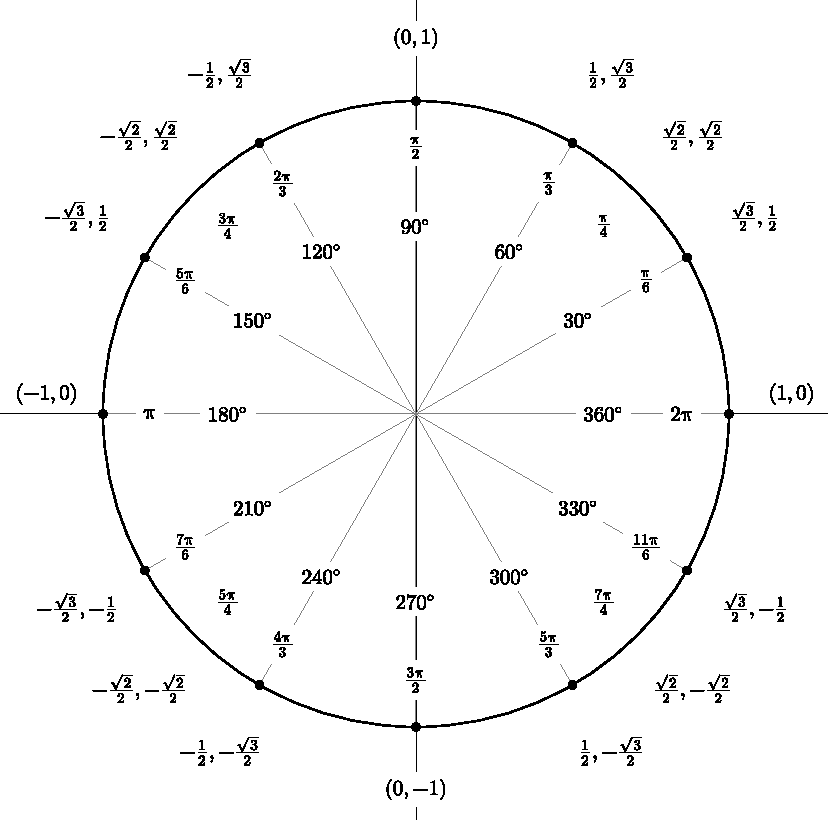
\includegraphics[width=\linewidth]{include_degrees_circle.pdf}
  
\end{center}

\section{Tabellen}
\subsection{Ableitungen}
\begin{center}
  % the c>{\centering\arraybackslash}X is a workaround to have a column fill up all space and still be centered
  \begin{tabularx}{\linewidth}{c>{\centering\arraybackslash}Xc}
    \toprule
    $\mathbf{F(x)}$ & $\mathbf{f(x)}$ & $\mathbf{f'(x)}$ \\
    \midrule
    $\frac{x^{-a+1}}{-a+1}$ & $\frac{1}{x^a}$ & $\frac{a}{x^{a+1}}$ \\
    $\frac{x^{a+1}}{a+1}$ & $x^a \ (a \ne 1)$ & $a \cdot x^{a-1}$ \\
    $\frac{1}{k \ln(a)}a^{kx}$ & $a^{kx}$ & $ka^{kx} \ln(a)$ \\
    $\ln |x|$ & $\frac{1}{x}$ & $-\frac{1}{x^2}$ \\
    $\frac{2}{3}x^{3/2}$ & $\sqrt{x}$ & $\frac{1}{2\sqrt{x}}$\\
    $-\cos(x)$ & $\sin(x)$ & $\cos(x)$ \\
    $\sin(x)$ & $\cos(x)$ & $-\sin(x)$ \\
    $\frac{1}{2}(x-\frac{1}{2}\sin(2x))$ & $\sin^2(x)$ & $2 \sin(x)\cos(x)$ \\
    $\frac{1}{2}(x + \frac{1}{2}\sin(2x))$ & $\cos^2(x)$ & $-2\sin(x)\cos(x)$ \\
    \multirow{2}*{$-\ln|\cos(x)|$} & \multirow{2}*{$\tan(x)$} & $\frac{1}{\cos^2(x)}$  \\
    & & $1 + \tan^2(x)$ \\
    $\cosh(x)$ & $\sinh(x)$ & $\cosh(x)$ \\
    $\log(\cosh(x))$ & $\tanh(x)$ & $\frac{1}{\cosh^2(x)}$ \\
    $\ln | \sin(x)|$ & $\cot(x)$ & $-\frac{1}{\sin^2(x)}$ \\
    $\frac{1}{c} \cdot e^{cx}$ & $e^{cx}$ & $c \cdot e^{cx}$ \\
    $x(\ln |x| - 1)$ & $\ln |x|$ & $\frac{1}{x}$ \\
    $\frac{1}{2}(\ln(x))^2$ & $\frac{\ln(x)}{x}$ & $\frac{1 - \ln(x)}{x^2}$ \\
    $\frac{x}{\ln(a)} (\ln|x| -1)$ & $\log_a |x|$ & $\frac{1}{\ln(a)x}$ \\
    \bottomrule
  \end{tabularx}
\end{center}
\subsection{Weitere Ableitungen}
\begin{center}
  \begin{tabularx}{\linewidth}{>{\centering\arraybackslash}X>{\centering\arraybackslash}X}
    \toprule
    $\mathbf{F(x)}$ & $\mathbf{f(x)}$ \\
    \midrule
    $\arcsin(x)$ & $\frac{1}{\sqrt{1 - x^2}}$ \\
    $\arccos(x)$ & $\frac{-1}{\sqrt{1 - x^2}}$ \\
    $\arctan(x)$ & $\frac{1}{1 + x^2}$ \\ 
    $x^x \ (x > 0)$ & $x^x \cdot (1 + \ln x)$ \\
    \bottomrule
  \end{tabularx}
\end{center}
\subsection{Integrale}
\begin{center}
  \begin{tabularx}{\linewidth}{>{\centering\arraybackslash}X>{\centering\arraybackslash}X}
    \toprule
    $\mathbf{f(x)}$ & $\mathbf{F(x)}$ \\
    \midrule
    $\int f'(x) f(x) \dx$ & $\frac{1}{2}(f(x))^2$ \\
    $\int \frac{f'(x)}{f(x)} \dx$ & $\ln|f(x)|$ \\
    $\int_{-\infty}^\infty e^{-x^2} \dx$ & $\sqrt{\pi}$ \\
    $\int (ax+b)^n \dx$ & $\frac{1}{a(n+1)}(ax+b)^{n+1}$ \\
    $\int x(ax+b)^n \dx$ & $\frac{(ax+b)^{n+2}}{(n+2)a^2} - \frac{b(ax+b)^{n+1}}{(n+1)a^2}$ \\
    $\int (ax^p+b)^n x^{p-1} \dx$ & $\frac{(ax^p+b)^{n+1}}{ap(n+1)}$ \\
    $\int (ax^p + b)^{-1} x^{p-1} \dx$ & $\frac{1}{ap} \ln |ax^p + b|$ \\
    $\int \frac{ax+b}{cx+d} \dx$ & $\frac{ax}{c} - \frac{ad-bc}{c^2} \ln |cx +d|$ \\
    $\int \frac{1}{x^2+a^2} \dx$ & $\frac{1}{a} \arctan \frac{x}{a}$ \\
    $\int \frac{1}{x^2 - a^2} \dx$ & $\frac{1}{2a} \ln\left| \frac{x-a}{x+a} \right|$ \\
    $\int \sqrt{a^2+x^2} \dx $ & $\frac{x}{2}f(x) + \frac{a^2}{2}\ln(x+f(x))$ \\
    \bottomrule
  \end{tabularx}
\end{center}

% end of larger array spacing
\endgroup
\end{document}
